\documentclass[14pt]{extbook}
\usepackage{multicol, enumerate, enumitem, hyperref, color, soul, setspace, parskip, fancyhdr} %General Packages
\usepackage{amssymb, amsthm, amsmath, latexsym, units, mathtools} %Math Packages
\everymath{\displaystyle} %All math in Display Style
% Packages with additional options
\usepackage[headsep=0.5cm,headheight=12pt, left=1 in,right= 1 in,top= 1 in,bottom= 1 in]{geometry}
\usepackage[usenames,dvipsnames]{xcolor}
\usepackage{dashrule}  % Package to use the command below to create lines between items
\newcommand{\litem}[1]{\item#1\hspace*{-1cm}\rule{\textwidth}{0.4pt}}
\pagestyle{fancy}
\lhead{Progress Quiz 5}
\chead{}
\rhead{Version C}
\lfoot{8497-6012}
\cfoot{}
\rfoot{Summer C 2021}
\begin{document}

\begin{enumerate}
\litem{
Solve the equation below. Then, choose the interval that contains the solution.\[ -7(-12x + 16) = -11(-18x + 10) \]\begin{enumerate}[label=\Alph*.]
\item \( x \in [-1.11, 0.07] \)
\item \( x \in [1.75, 2.12] \)
\item \( x \in [0.51, 1.13] \)
\item \( x \in [-2.42, -1.94] \)
\item \( \text{There are no real solutions.} \)

\end{enumerate} }
\litem{
Write the equation of the line in the graph below in Standard Form $Ax+By=C$. Then, choose the intervals that contain $A, B, \text{ and } C$.
\begin{center}
    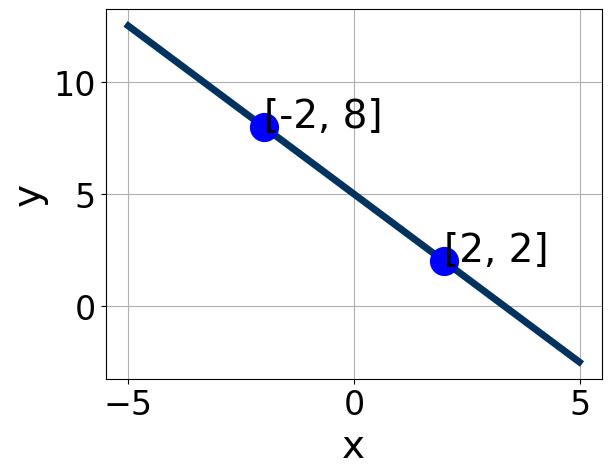
\includegraphics[width=0.5\textwidth]{../Figures/linearGraphToStandardCopyC.png}
\end{center}
\begin{enumerate}[label=\Alph*.]
\item \( A \in [2.19, 3.42], \hspace{3mm} B \in [-2.33, -1.88], \text{ and } \hspace{3mm} C \in [-10, -7] \)
\item \( A \in [-3.05, -2.74], \hspace{3mm} B \in [-2.33, -1.88], \text{ and } \hspace{3mm} C \in [-10, -7] \)
\item \( A \in [1.38, 1.84], \hspace{3mm} B \in [-1.72, -0.83], \text{ and } \hspace{3mm} C \in [-8, -1] \)
\item \( A \in [1.38, 1.84], \hspace{3mm} B \in [0.74, 1.51], \text{ and } \hspace{3mm} C \in [0, 8] \)
\item \( A \in [2.19, 3.42], \hspace{3mm} B \in [1.77, 2.43], \text{ and } \hspace{3mm} C \in [10, 12] \)

\end{enumerate} }
\litem{
Solve the equation below. Then, choose the interval that contains the solution.\[ -8(-7x -19) = -4(-14x + 9) \]\begin{enumerate}[label=\Alph*.]
\item \( x \in [-0.3, 0.5] \)
\item \( x \in [-1.4, -0.4] \)
\item \( x \in [-0.3, 0.5] \)
\item \( x \in [-0.3, 0.5] \)
\item \( \text{There are no real solutions.} \)

\end{enumerate} }
\litem{
Solve the linear equation below. Then, choose the interval that contains the solution.\[ \frac{-7x -4}{6} - \frac{-3x -9}{2} = \frac{-9x -5}{8} \]\begin{enumerate}[label=\Alph*.]
\item \( x \in [-8.7, -6.2] \)
\item \( x \in [-3.8, -1.8] \)
\item \( x \in [1.8, 3.5] \)
\item \( x \in [-1.1, -0.6] \)
\item \( \text{There are no real solutions.} \)

\end{enumerate} }
\litem{
First, find the equation of the line containing the two points below. Then, write the equation in the form $ y=mx+b $ and choose the intervals that contain $m$ and $b$.\[ (2, 5) \text{ and } (-2, 10) \]\begin{enumerate}[label=\Alph*.]
\item \( m \in [-1.7, -0.9] \hspace*{3mm} b \in [7.2, 8.2] \)
\item \( m \in [-1.7, -0.9] \hspace*{3mm} b \in [2.1, 5.2] \)
\item \( m \in [-1.7, -0.9] \hspace*{3mm} b \in [10, 12.1] \)
\item \( m \in [-1.7, -0.9] \hspace*{3mm} b \in [-10, -6] \)
\item \( m \in [-0.4, 2.5] \hspace*{3mm} b \in [12.3, 16.7] \)

\end{enumerate} }
\litem{
Find the equation of the line described below. Write the linear equation in the form $ y=mx+b $ and choose the intervals that contain $m$ and $b$.\[ \text{Parallel to } 3 x - 7 y = 13 \text{ and passing through the point } (-5, 6). \]\begin{enumerate}[label=\Alph*.]
\item \( m \in [-0.11, 2.33] \hspace*{3mm} b \in [11, 15] \)
\item \( m \in [-0.11, 2.33] \hspace*{3mm} b \in [7.14, 10.14] \)
\item \( m \in [2.01, 2.58] \hspace*{3mm} b \in [7.14, 10.14] \)
\item \( m \in [-0.11, 2.33] \hspace*{3mm} b \in [-12.14, -6.14] \)
\item \( m \in [-0.52, 0.19] \hspace*{3mm} b \in [-3.14, 5.86] \)

\end{enumerate} }
\litem{
Solve the linear equation below. Then, choose the interval that contains the solution.\[ \frac{9x + 7}{6} - \frac{-3x + 4}{5} = \frac{6x + 5}{3} \]\begin{enumerate}[label=\Alph*.]
\item \( x \in [-0.78, 4.22] \)
\item \( x \in [12, 15] \)
\item \( x \in [-3, -2] \)
\item \( x \in [19, 26] \)
\item \( \text{There are no real solutions.} \)

\end{enumerate} }
\litem{
First, find the equation of the line containing the two points below. Then, write the equation in the form $ y=mx+b $ and choose the intervals that contain $m$ and $b$.\[ (-4, -3) \text{ and } (-11, -9) \]\begin{enumerate}[label=\Alph*.]
\item \( m \in [-2.37, 0.6] \hspace*{3mm} b \in [-20.1, -18] \)
\item \( m \in [0.58, 2.01] \hspace*{3mm} b \in [-1.51, -0.35] \)
\item \( m \in [0.58, 2.01] \hspace*{3mm} b \in [1.45, 2.02] \)
\item \( m \in [0.58, 2.01] \hspace*{3mm} b \in [0.67, 1.58] \)
\item \( m \in [0.58, 2.01] \hspace*{3mm} b \in [-0.22, 0.91] \)

\end{enumerate} }
\litem{
Write the equation of the line in the graph below in Standard Form $Ax+By=C$. Then, choose the intervals that contain $A, B, \text{ and } C$.
\begin{center}
    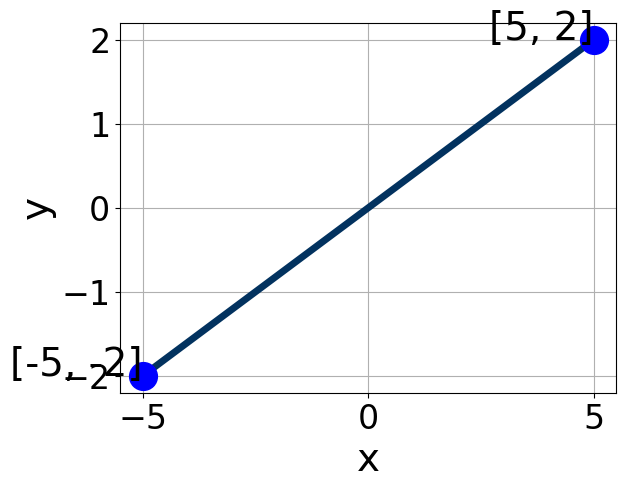
\includegraphics[width=0.5\textwidth]{../Figures/linearGraphToStandardC.png}
\end{center}
\begin{enumerate}[label=\Alph*.]
\item \( A \in [-1.2, 0.4], \hspace{3mm} B \in [0.08, 1.32], \text{ and } \hspace{3mm} C \in [-1, 5] \)
\item \( A \in [1.8, 3.9], \hspace{3mm} B \in [-5.9, -3.95], \text{ and } \hspace{3mm} C \in [-1, 5] \)
\item \( A \in [1.8, 3.9], \hspace{3mm} B \in [3.04, 5.46], \text{ and } \hspace{3mm} C \in [-1, 5] \)
\item \( A \in [-1.2, 0.4], \hspace{3mm} B \in [-1.68, -0.26], \text{ and } \hspace{3mm} C \in [-1, 5] \)
\item \( A \in [-2.8, -0.5], \hspace{3mm} B \in [3.04, 5.46], \text{ and } \hspace{3mm} C \in [-1, 5] \)

\end{enumerate} }
\litem{
Find the equation of the line described below. Write the linear equation in the form $ y=mx+b $ and choose the intervals that contain $m$ and $b$.\[ \text{Parallel to } 3 x + 5 y = 8 \text{ and passing through the point } (9, -7). \]\begin{enumerate}[label=\Alph*.]
\item \( m \in [-2.89, -0.85] \hspace*{3mm} b \in [-4.4, -0.3] \)
\item \( m \in [-1.24, -0.43] \hspace*{3mm} b \in [-4.4, -0.3] \)
\item \( m \in [-1.24, -0.43] \hspace*{3mm} b \in [0.6, 3.5] \)
\item \( m \in [-1.24, -0.43] \hspace*{3mm} b \in [-16.6, -15.7] \)
\item \( m \in [-0.11, 1.28] \hspace*{3mm} b \in [-12.5, -11.9] \)

\end{enumerate} }
\end{enumerate}

\end{document}